%%%%%%%%%%%%%%%%%%%%%%%%%%%%%%%%%%%%%%%%%%
%%%%%%%%%%%%%                 %%%%%%%%%%%%
%%%%%%%%%%%%%    EXERCISE 1   %%%%%%%%%%%%
%%%%%%%%%%%%%                 %%%%%%%%%%%%
%%%%%%%%%%%%%%%%%%%%%%%%%%%%%%%%%%%%%%%%%%
\begin{exercise}[BAYES NETWORK ]{Evaluate the distributions p(a),p(b|c),and p(c|a) corresponding to the joint distribution given in Table 1. Hence show by direct evaluation that p(a,b,c) = p(a)p(c|a)p(b|c). Draw the corresponding directed graph (30)
    \begin{figure}[ht]
        \centering
        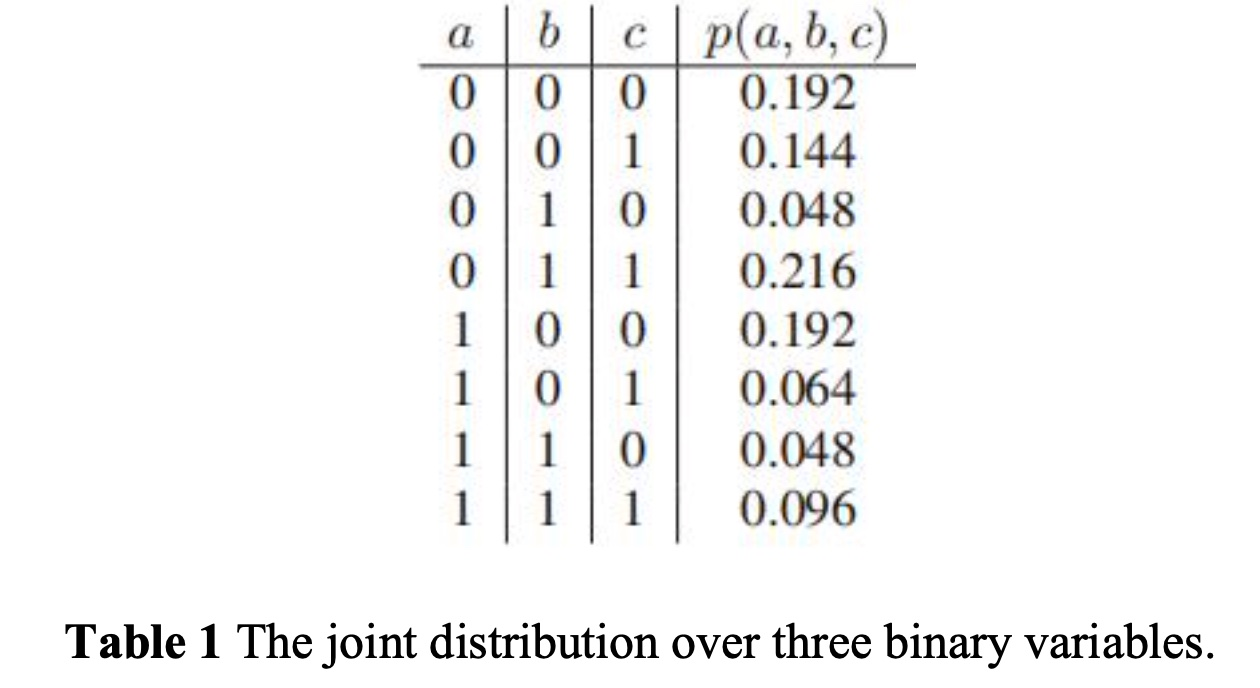
\includegraphics[width=8cm]{img/ex3-1.jpg}
    \end{figure}
    }
  \begin{solution}
  \par{~}
  The directed graph is shown below, and the distributions are listed on the next page.

  \begin{figure}[ht]
        \centering
        
\includegraphics[width=8cm]{img/ex3-5.jpg}
    \end{figure}


  \begin{table}[p]
    \centering
    \begin{tabular}{cc}
    \hline
    a & p(a) \\ \hline
    0 & 0.6  \\
    1 & 0.4  \\ \hline
    \end{tabular}


\begin{tabular}{ccc}
    \hline
    b & c & p(b|c) \\ \hline
    0 & 0 & 0.8    \\
    1 & 0 & 0.2    \\
    0 & 1 & 0.4    \\
    1 & 1 & 0.6    \\ \hline
    \end{tabular}

\begin{tabular}{ccc}
    \hline
    a & c & p(c|a) \\ \hline
    0 & 0 & 0.4    \\
    0 & 1 & 0.6    \\
    1 & 0 & 0.6    \\
    1 & 1 & 0.4    \\ \hline
    \end{tabular}

\begin{tabular}{ccccccc}
    \hline
    a & b & c & p(a) & p(c|a) & p(b|c) & p(a,b,c) \\ \hline
    0 & 0 & 0 & 0.6  & 0.4    & 0.8    & 0.192    \\
    0 & 0 & 1 & 0.6  & 0.6    & 0.4    & 0.144    \\
    0 & 1 & 0 & 0.6  & 0.4    & 0.2    & 0.048    \\
    0 & 1 & 1 & 0.6  & 0.6    & 0.6    & 0.216    \\
    1 & 0 & 0 & 0.4  & 0.6    & 0.8    & 0.192    \\
    1 & 0 & 1 & 0.4  & 0.4    & 0.4    & 0.064    \\
    1 & 1 & 0 & 0.4  & 0.6    & 0.2    & 0.048    \\
    1 & 1 & 1 & 0.4  & 0.4    & 0.6    & 0.096    \\ \hline
    \end{tabular}
\end{table}


  \end{solution}
  \label{ex1}
\end{exercise}


\newpage


%%%%%%%%%%%%%%%%%%%%%%%%%%%%%%%%%%%%%%%%%%
%%%%%%%%%%%%%                 %%%%%%%%%%%%
%%%%%%%%%%%%%    EXERCISE 2   %%%%%%%%%%%%
%%%%%%%%%%%%%                 %%%%%%%%%%%%
%%%%%%%%%%%%%%%%%%%%%%%%%%%%%%%%%%%%%%%%%%
\begin{exercise}[]{Markov Model Use the technique of d-separation, to verify that the Markov model shown in Figure 1 having $\mathrm{N}$ nodes in total satisfies the conditional independence properties
    $$
    p\left(\boldsymbol{x}_{n} \mid \boldsymbol{x}_{1}, \ldots, \boldsymbol{x}_{n-1}\right)=p\left(\boldsymbol{x}_{n} \mid \boldsymbol{x}_{n-1}\right)
    $$
    for $\mathrm{n}=2$,.,N. Similarly, show that a model described by the graph in Figure 2 in which there are $\mathrm{N}$ nodes in total (30)

    \begin{figure}[h]
        \centering
        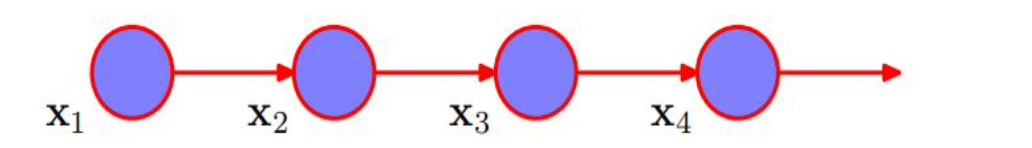
\includegraphics[width=8cm]{img/ex3-2.jpg}
        \caption{A first-order Markov chain of observations $\left\{x_{n}\right\}$ in which the distribution $p\left(x_{n} \mid x_{n-1}\right)$ of a particular observation $x_{n}$ is conditioned on the value of the previous observation $x_{n-1}$}
    \end{figure}

    \begin{figure}[h]
        \centering
        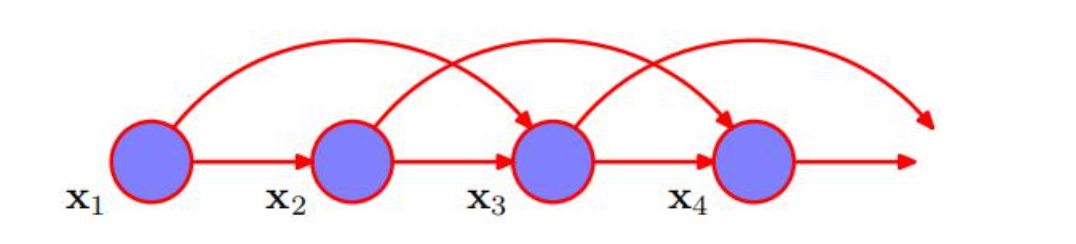
\includegraphics[width=8cm]{img/ex3-3.jpg}
        \caption{A second-order Markov chain, in which the conditional distribution of a particular observation $x_{n}$ depends on the values of the two previous observations $x_{n-1}$ and $x_{n-2}$.
        }
    \end{figure}
    
    }
  \begin{solution}
  \par{~}
  For second-order Markov Chain, we assert that $X_{N} \perp X_{N-3}, \ldots, X_{1} | X_{N-2}, X_{N-1}$, i.e. 
  $$
    p\left(\boldsymbol{x}_{n} \mid \boldsymbol{x}_{1}, \ldots, \boldsymbol{x}_{n-1}\right)=p\left(\boldsymbol{x}_{n} \mid \boldsymbol{x}_{n-1}, \boldsymbol{x}_{n-2}\right)
    $$
  \end{solution}

  For every $X_i, i < N - 2$, we check the undirected path in the graph between $X_i$ and $X_N$. Note that it must pass through either $X_{N-1}$ or $X_{N-2}$, forming a casual relation. Since $X_{N-1}$ and $X_{N-2}$ colored grey, all the paths between $X_i$ and $X_N$ are inactive. Thus, by d-separation, the assertion holds.
  \label{ex2}
\end{exercise}


\newpage

%%%%%%%%%%%%%%%%%%%%%%%%%%%%%%%%%%%%%%%%%%
%%%%%%%%%%%%%                 %%%%%%%%%%%%
%%%%%%%%%%%%%    EXERCISE 3   %%%%%%%%%%%%
%%%%%%%%%%%%%                 %%%%%%%%%%%%
%%%%%%%%%%%%%%%%%%%%%%%%%%%%%%%%%%%%%%%%%%
\begin{exercise}[HMM]{ Consider the following Hidden Markov Model. $O_1$ and $O_2$ are supposed to be shaded.  Suppose that we observe $O_{1}=a$ and $O_{2}=b$ Using the forward algorithm, compute the probability distribution $P\left(W_{2} \mid O_{1}=a, O_{2}=b\right)$ one step at a time. (40)
    \begin{enumerate}
        \item Compute $\mathrm{P}\left(W_{1}, O_{1}=a\right)$.
        \item Using the previous calculation,compute $\mathrm{P}\left(\mathrm{W}_{2}, \mathrm{O}_{1}=a\right)$
        \item Using the previous calculation,compute $\mathrm{P}\left(\mathrm{W}_{2}, \mathrm{O}_{1}=a, \mathrm{O}_{2}=b\right)$
        \item Finally, compute $P\left(W_{2} \mid O_{1}=a, O_{2}=b\right)$.
    \end{enumerate}

    \begin{figure}[h]
        \centering
        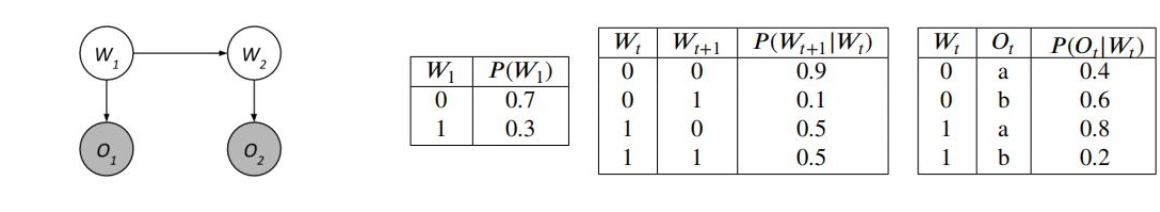
\includegraphics[width=12cm]{img/ex3-4.jpg}
    \end{figure}
        }
  \begin{solution}
  \par{~}
  \end{solution}
  \label{ex3}
\end{exercise}